\documentclass[times, utf8, seminar, numeric]{fer}
\usepackage{booktabs}
 \usepackage{url}
\usepackage{algorithm}
\usepackage[noend]{algpseudocode}

\makeatletter
\renewcommand{\ALG@name}{Algoritam}
\makeatother

\begin{document}

% Ukljuci literaturu u seminar
\nocite{*}

% TODO: Navedite naslov rada.
\title{Rješavanje problema rubikove kocke evolucijskim algoritmima}

% TODO: Navedite vaše ime i prezime.
\author{Vinko Kolobara}

% TODO: Navedite ime i prezime voditelja.
\voditelj{Domagoj Jakobović}

\maketitle

\tableofcontents

\chapter{Uvod}
Uvod.

\chapter{Problem rubikove kocke}
\section{Definicija}


\begin{figure}[h]
\centering
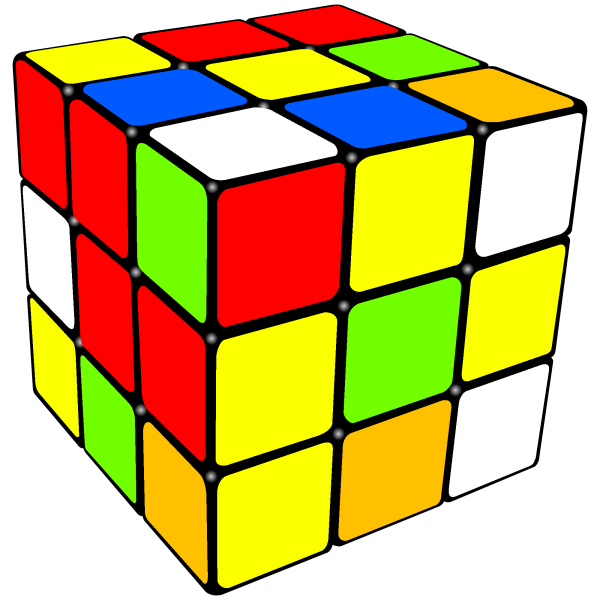
\includegraphics[width=0.45\textwidth]{image/scrambled_rubik's_cube.png}
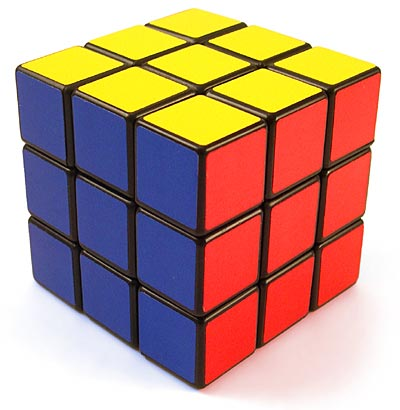
\includegraphics[width=0.45\textwidth]{image/rubik_cube_goal_state.jpg}
\caption{Primjer nekog nasumičnog početnog stanja rubikove kocke (lijeva slika) i prikaz ciljnog stanja (desna slika) }
\end{figure}

Rubikova kocka je logička igra općenito dimenzija $N\times N\times N$ u kojoj je cilj pomoću osnovnih rotacija strana kocke postići da svaka strana bude iste boje. U ovom radu će se nadalje govoriti o kocki dimenzija $3\times3\times3$. Za svaku stranu moguće su dvije vrste rotacije, u smjeru kazaljke na satu i obrnuto. Sve dozvoljene rotacije označavat će se:

\begin{itemize}
\item F - prednja strana u smjeru kazaljke sata, 
\item F' - prednja strana obrnuto od kazaljke sata
\item B - stražnja strana u smjeru kazaljke sata, 
\item B' - stražnja strana obrnuto od kazaljke sata
\item U - gornja strana u smjeru kazaljke sata, 
\item U' - gornja strana obrnuto od kazaljke sata
\item D - donja strana u smjeru kazaljke sata, 
\item D' - donja strana obrnuto od kazaljke sata
\item L - lijeva strana u smjeru kazaljke sata, 
\item L' - lijeva strana obrnuto od kazaljke sata
\item R - desna strana u smjeru kazaljke sata, 
\item R' - desna strana obrnuto od kazaljke sata
\end{itemize}

Često se uvode i dodatne rotacije, koje označavaju uzastopno izvođenje jedne od jednostavnih rotacija:
\begin{itemize}
\item F2 - prednja strana dva puta u smjeru kazaljke sata, 
\item B2 - stražnja strana dva puta u smjeru kazaljke sata, 
\item U2 - gornja strana dva puta u smjeru kazaljke sata, 
\item D2 - donja strana dva puta u smjeru kazaljke sata, 
\item L2 - lijeva strana dva puta u smjeru kazaljke sata, 
\item R2 - desna strana dva puta u smjeru kazaljke sata
\end{itemize}

Svaka strana se može prikazati kao $NxN$ matrica sa određenim bojama na poljima. Dodatno, može se uvesti i pojam kockice \engl{cubie}, i to dvije vrste, kutna \engl{Corner Cubie} i rubna \engl{Edge Cubie}. Svaka kutna kockica na sebi ima 3 boje, i može biti u 2 osnovna stanja: ispravno orijentirana (kada su sve boje na pravim mjestima) i pogrešno orijentirana. Svaka rubna kockica sastoji se od 2 boje, i može biti u ista 2 stanja kao i kutna. 
Na kocki postoji 8 kutnih i 12 rubnih kockica.

%SLIKA EDGE I CORNER CUBIE


Broj stanja u kojima se rubikova kocka može naći iznosi oko 43 kvintilijuna što je popriličan broj i obična metoda grubom silom bi bila neuspješna. Zbog toga postoje brojni uspješni algoritmi kojima se može brzo i efikasno doći do rješenja.

Najuspješniji algoritmi koriste teoriju grupa i činjenicu da kada dođu u određeni skup stanja (grupu), ako se uzme određeni podskup rotacija, nemoguće je "pogoršati" rješenje već samo prijeći u sljedeću grupu u kojoj ima manje stanja i koja je bliža ciljnom rješenju. Primjeri takvih algoritama su Thistlewaite, Kociemba, Korf\dots

Kako je ovo kombinatorni problem i jako složen za uobičajeno rješavanje, pokušaj u ovom seminaru bit će usmjeren na rješavanje rubikove kocke upotrebon samo evolucijskih algoritama, bez korištenja dodatnih informacija iz teorije grupa i sličnog.

\section{Programska reprezentacija}


\chapter{Genetski algoritam}
Ukratko što je GA i primjena na rubikovu kocku.

\section{Opis genetskog algoritma}
Genetski algoritam pripada evolucijskim algoritmima i pokušava korištenjem genetskih operatora (križanje, mutacija, selekcija) doći do rješenja problema. Sastoji se od populacije od $N$ jedinki, svaka jedinka sadrži mjeru sposobnosti \engl{fitness} koja označava koliko je ta jedinka blizu ciljnom rješenju, a svaka jedinka se sastoji od $m$ gena koji predstavljaju dio rješenja. 

Selekcijom biramo roditelje za križanje, križamo ih, obavljamo mutaciju i to sve ponavljamo dok se ne ostvari uvjet zaustavljanja (obično broj iteracija ili pronalazak rješenja ili dostignuta određena mjera sposobnosti).

\begin{algorithm}
\begin{algorithmic}[1]
\renewcommand{\algorithmicwhile}{\textbf{dok}}
\renewcommand{\algorithmicdo}{\textbf{radi}}

\caption{Primjer eliminacijskog genetskog algoritma}

\State P <- generiraj nasumično početnu populaciju
\While{nije zadovoljen uvjet zaustavljanja}
	\State R1, R2, W <- selekcija(P) \Comment{Izaberi 2 roditelja i jedinku za eliminaciju}
	\State D <- križaj(R1, R2) 
	\State D <- mutiraj(D)
	\State P(W) <- D \Comment{Zamijeni najgoreg novonastalim djetetom}
\EndWhile
\end{algorithmic}
\end{algorithm}

\section{Primjena GA na problem rubikove kocke}

\subsection{Reprezentacija rješenja}
Poznato je da se svaka rubikova kocka može riješiti u maksimalno 20 rotacija, zato će svaka jedinka biti predstavljena kao niz od 40 gena (cijelih vrijednosti) koji predstavljaju, redom, slijed rotacija koje je potrebno izvesti. Dozvoljeni brojevi za svaki gen su iz raspona $[0, 17]$.
Vrijednosti iz raspona $[0, 12]$ predstavljaju obične operacije (rotacija svake strane u bilo kojem smjeru), dok vrijednosti iz raspona $[13, 17]$ predstavljaju složene operacije (dvostruke rotacije pojedine strane).

%OVDJE UBACI PRIMJER RJEŠENJA

\subsection{Genetski operatori i mjera sposobnosti}
Korištena je troturnirska selekcija, za križanje je korišteno križanje s jednom i dvije točke prekida, a za mutaciju je implementiran poseban operator.
Koristi se operator mutacije koji će odrediti nakon koje je rotacije u kromosomu najbolje stanje kocke, i sve rotacije nakon tog stanja nasumično generira.

Posebnost ovog problema i ovakve implementacije operatora je to što se mutacija i križanje ne koriste u kontekstu u kojem se inače koriste u genetskom algoritmu. Naime, križanje uobičajeno ne mijenja previše rješenje i služi za lokalno pretraživanje prostora stanja, a mutacija je zadužena da rješenje odvede u sasvim drugom smjeru. U ovom slučaju, događa se upravo obrnuta stvar, križanje obavlja posao mutacije, a mutacija posao križanja.

Implementirane su dvije različite mjere sposobnosti. 
Prva mjera sposobnosti jednostavno broji koliko je boja na pravim mjestima kocke (ne brojeći centralni element svake strane jer je on fiksan). Maksimalna vrijednost ove mjere je 48.

Druga mjera broji koliko je kutnih i rubnih kockica na pravim mjestima u pravoj orijentaciji. Maksimalna vrijednost ove mjere je 96 (svaka ispravna rubna kockica vrijedi 4, dok svaka ispravna kutna kokckica vrijedi 6, napravljeno za to da u slučaju kombinacije sa prvom mjerom svaka podmjera sudjeluje u jednakom broju).

%UBACI PRIMJER RJEŠENJA I MJERA SPOSOBNOSTI

\chapter{Genetsko programiranje}
Ukratko što je GP i primjena na rubikovu kocku.

\section{Opis genetskog programiranja}
Genetsko programiranje također pripada evolucijskim algoritmima i koristi iste funkcije kao i genetski algoritam. Najveća razlika je prikaz rješenja. U genetskom algoritmu se rješenje uglavnom prikazuje kao niz gena, dok se u genetskom programiranju rješenje prikazuje kao stablo. Svako stablo se sastoji od funkcijskih \engl{Function} i završnih \engl{Terminal} čvorova. Završni čvorovi se nalaze u listovima stabla, dok funkcijski nešto rade sa podstablima kako bi odredili konačan rezultat.

Rad algoritma je jednak genetskom, uz uvođenje dodatnih složenosti kod stvaranja inicijalne populacije te složenijih operatora križanja i mutacije.

%PRIMJER GP STABLA

\section{Primjena GP na problem rubikove kocke}
Pokušaj genetskim programiranjem, za razliku od prethodnog pokušaja, za cilj ima pronaći najbolji program koji će u što manje koraka riješiti bilo koju konfiguraciju kocke, točnije, moći će odrediti najbolju rotaciju (ili niz rotacija) za bilo koje stanje kocke. 

Potrebno je definirati dodatne funkcije, koje će za svaku rubnu ili kutnu kockicu odrediti je li na pravom mjestu ili ne. Ovisno o tome, funkcija će izvesti lijevo ili desno podstablo. 

Završni čvorovi će biti cijeli brojevi koji predstavljaju operaciju koja se treba izvršiti.

Svaki program se izvodi dok ne dođe do rješenja rubikove kocke ili dok dosegne dozvoljeni broj rotacija (50).

Korištene mjere sposobnosti su iste kao za genetski algoritam, uz to što se dodatno nagradi algoritam koji je prije došao do rješenja.



\chapter{Rezultati}
Opiši poražavajuće rezultate...

\chapter{Zaključak}
Zaključi nešto.

\bibliography{literatura}
\bibliographystyle{fer}

\chapter{Sažetak}
Sažetak.

\end{document}
